\documentclass[titlepage]{article}
\usepackage{amsmath}
\usepackage[utf8]{inputenc}
\usepackage{graphicx}

\author{Jan Alexander Bremnes\\Magnus Kirø}
\title{IT3105 - Ex 2\\Voice Recognition}
\date{October 2011}

\begin{document}

    \maketitle
    \tableofcontents
    \pagenumbering{arabic}
    \graphicspath{{SRS/img/}}
    \newpage

\section{Introduction}
In this report we will discuss the process of speech recognition, a project in the course IT3105 - AI programming. The project consisted of creating a single word speech recognition program, capable of recognising words from a vocabulary consisting of four words. We were given a set of training data, several recordings of the specific words, that should be used to train the system, and then we were supposed to test it with another set of recordings of the same words. To achieve this, we were supposed to use hidden Markov models(HMM) as a key component in our calculations. HMMs are common in speech recognition, and quite useful in many other cases. 

As implementation tool for the project we used MATLAB and its programming language. It was recommended to use MATLAB because the implementation was going to be related to signal processing and matrix calculations. Both are fields in which MATLAB is really powerful.

\section{System Description}
    Unfortunately, we were not able to complete the project, so we do not have a working system. We managed to get as far as to the E-step in the learning part (section 2.3, page.17 of the Lecture Notes), but encountered a problem when trying to reestimate the value for sigma. Because of this, the models does not get updated properly when doing the forward and backwards passes. We did not manage to locate and fix the error before running out of time.

\subsection{Code Files and what they do}
\newline
\begin{itemize}
    \item[main.m] Main first create a set of models, one for each word, with number of states in each model equal to the number of phonems in the word to be modelled.  It imports the wav-files anduse preparedSignal to create the datastructure we want to represent our data. All the processed wav-files are added to a three dimensional array, before doing one forward pass on each. Then learn.m is called to do forward and backward passes on each file until we reach convergence.
    
\item[prepareSignal.m] prepareSignal contains the code to manipulate the data from the .wav files to a more useful representation. Fist we find the length of the window we want to use and normalize the input sound data before we create the matrix of frames with 80 samples per frame and 50 percent overlap. Then we smooth the frame with a hamming window, before applying the discrete Fourier Transform on the framed and smoothed signal. Then we use findpeaks to specify points of data to identify the specific word. We select the n largest peaks pr frame.  

\item[classifier.m] We run our classifier independantly of the learning process. It reads all the query files and the models trained by main.m. The classifier uses the data recorded when training the models. This data is stored in a file, models.mat, and loaded in to MATLAB when we are going to classify the query files. Classify calls the forward(HMM) with the data to be classified and the model it is being compared to. Forward(HMM) then returns the probability that the model and the data is the same word. Classify finds the highest the most probable word for all the query files and returns an array of the result at the end. 


\item[hmm.m] This class constructs a Hidden Markov Model. Its name is the word the model shall represent and number of states is the number of phonems in that word. The model consists of an array containing the prior distribution, a NxN transition matrix, called dynModel, and the observationmodel, which consists of mu and sigma, and a single gaussian mixture for each state. 


\item[forward.m] Does forward passes over the data and calculates alpha for all obervations. And returns the probability that the data inut to this file is equal to the model input. 

\item[backward.m] Does backward passes and calculates beta for all observations.

\item[learn.m] This class is used to train the HMMs. It receives a data structure containing all the recordings of a single word, and the model representing that word. For every recording, it does forward and backward passes, then computes Xi and Gamma for all observations, using the alphas and betas received from forward.m and backward.m. Then the prior distribution and the transition model is updated, before updating mu and sigma.

\end{itemize}

\newpage
\section{Data Representation}
% How we represent the sound as data and why. 
% Results from the different parts si required. 
    % picture from part 1
    % picture from part 2
    % picture from part 3
    % picture from part 4
    \subsection{Data representation} 
    We import all the recordings for the given word, and make them equal length by padding them with zero values. Each recorded sound is split into frames, with each frame consisting of 80 consecutive datapoints from the original speech sample. The frames are smoothed with a hamming window, and the discrete Fourier Transform is applied. We then find the n largest peaks in each window, and store these values in an array of size n x no.frames. This is our representation of the speech sample. See fig.1 to see a plot of the result. All the samples of a word, is added as a page in a three dimensional array, which is then used to teach the HMMs.
We chose this structure for our data to be able to have all the data in one matrix. This makes operations on our structure easy with the matrix operations in MATLAB. We thought of using spectrograms early in the poject, but rejected them because we didn't find an easy way to use them.
We have no prior experience with signal processing, so we don't know very much about what parts of an audio signal that are interesting when implementing a robust representation, so our representation is somewhat the result of trial and error.  
\begin{figure}[Frames plotted]
     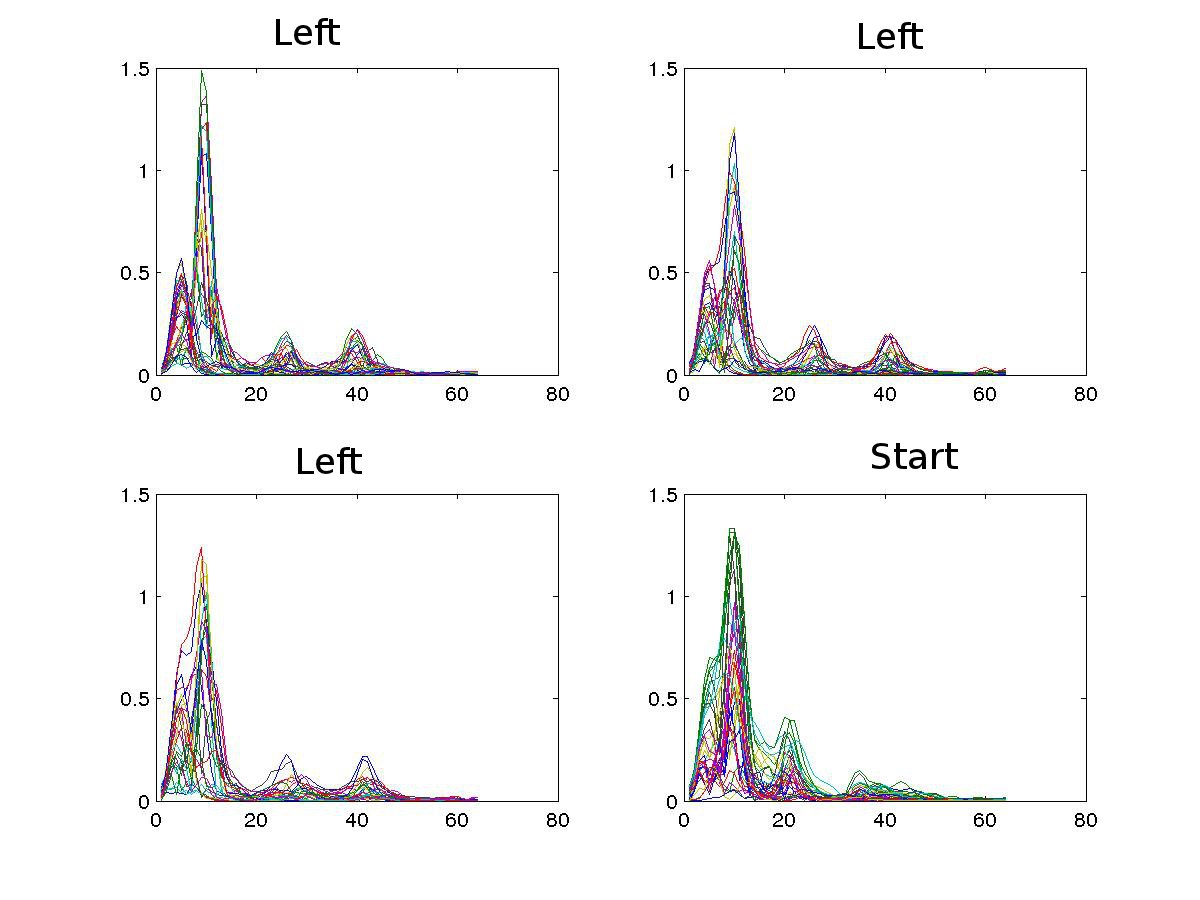
\includegraphics[scale=0.3]{leftleftleftgo}
    \caption{Three different utterances of "Left" and one of "Start"}
\end{figure}


    \subsection{HMM}
The HMM consists fo three main models, the prior, dynamic and observation models.  
We set the observation model as one multivariate Gaussian over the features per state of the hidden variable. This is the simple observation model. We could have chosen the observation model to be a mixture of Gaussians. We chose not to do this because of the more difficult implementation and due to time limitations. 
The priorHidden is an array containing the probabilities of each state in the model being the starting state; the point at which we enter the model.
The dynamic model (dynMod) is the transition matrix. It contains the probabilities of moving from state(i) to state(j).

\section{Test data classification and results}
        Because we were not able to finish the project, we do not have any results to show from the classification. The classifier is implemented, but since the models have not been trained, the results are useless, see fig.2
\begin{figure}[Frames plotted]
\center
     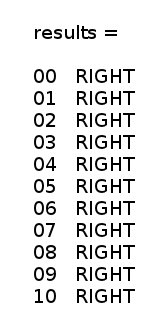
\includegraphics[scale = 0.5]{result}
    \caption{Sample output from Classifier}
\end{figure}
Our data representation is probably not good enough for accurate speech identification. There are very few features recorded per frame in the signal, because not all frames have an equal amount of peaks to be detected. To make it more robust, we can add different features, such as zero-point crossings etc. With a working system, we could have tested different kind of speech representation, and found the one with the best results. If the desired accuracy had not been reached, we could have looked into tried implmenting the most widely used representation of sound for speech recognition, the Mel-frequency spectrum coefficients. In addition to changing the representation speech, the system could probably have been improved by increasing the amount of training data for the HMMs.

\section{Conclusion}
        As already mentioned, our system does not work at the moment. We think we were able to implement Part 1 & Part 2 of the project, and some parts of Part 3, but we encountered some problems when trying to reestimate Sigma in the learning procedure. Since we were unable to locate the problem and fix it within the deadline of the project, we were unable to train the HMM models, and it is therefore difficult to judge the robustness of our representation of the speech signals. Most probably, they need quite a fair amount of adjustment, as the only features we extract are the n largest peaks for every frame in the signal. It has been a very educational experience, but we understand why it was recommended to have had the courses TDT4171 - Artificial Intelligence Methods, TDT4173 - Machine Learning and Case-based reasoning, in addition to some knowledge about matrix calculations and signal processing.

\end{document}
